%-------------------------------------------------------------------------
\section{Experiments and Results}  \label{Sec:Experiments}
We test our DeepPRT method against different animated objects: We animate a \textit{Pirate Head} and a \textit{Fish} object using a blendshape model and apply physically-based deformations to animate a \textit{Cloth} object.
\\
The mesh resolution of the objects is $256 \times 256$. However, for the Fish object we increase the resolution to $512 \times 512$ to avoid reconstruction artifacts (see figure \ref{Fig: Fish Reconstruction})
% FIGURE (Fish Resampling)
\begin{figure}[H]
  \centering
    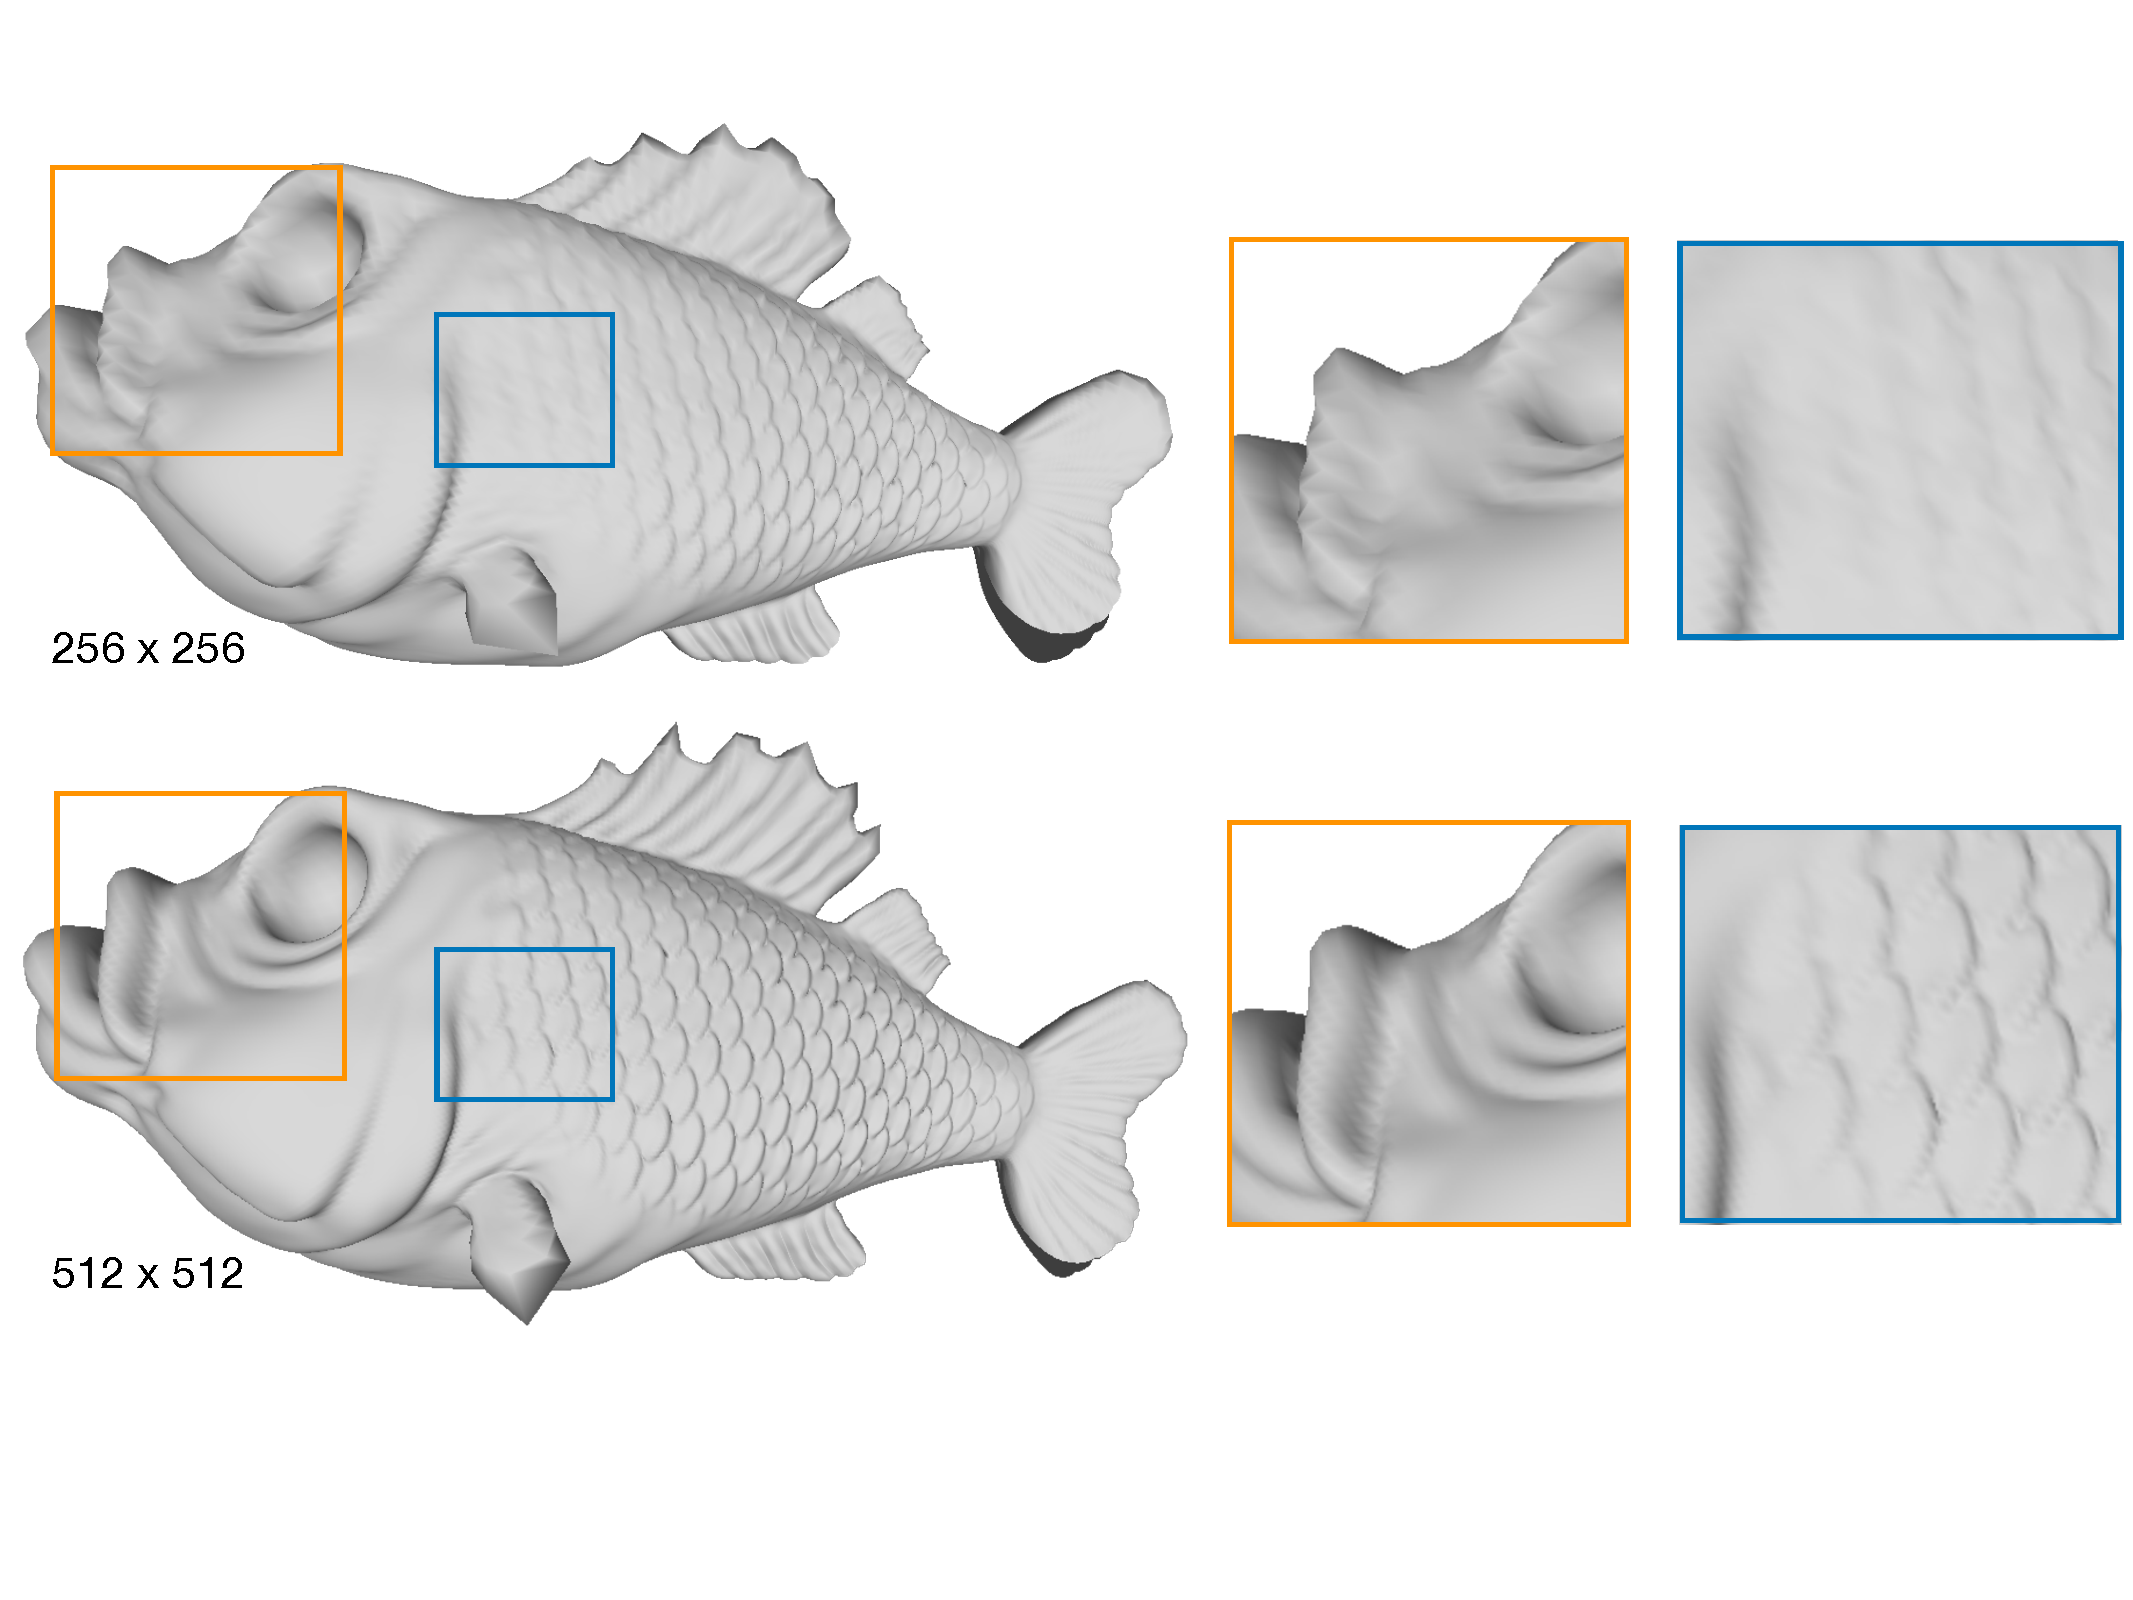
\includegraphics[width=0.4\textwidth]{Figures/fish}
     \caption{Fish reconstructions after regular sampling of squared harmonic map. \textit{Top:} Sampled by a $256 \times 256$ grid, shows detail loss and distortions. \textit{Bottom:} Higher sampling $512 \times 512$ needed to preserve detail and minimize artifacts.}
     \label{Fig: Fish Reconstruction}
\end{figure}~
This distortions arise due to the uniform remeshing, while using a sub-optimal choice of 2D surface parametrization (Harmonic Map), leading to poorly sampled surface areas in regions of higher curvatures. A more suited parametrization, that minimizes distortion after resampling, is the \textit{geometric-stretch} parametrization  \cite{gu2002geometry}.
%%%%%%%%%%%%%%%%%%%%%%%%%%%%%
% MEMORY and QUALITY
%%%%%%%%%%%%%%%%%%%%%%%%%%%%%
\subsection*{DeepPRT Quality and Memory Savings} \label{Sec: memory_savings}
For each of the test objects, our train- and validation sets together comprise 500 distinct object deformations. 
Within that deformation set, our U-Net model is able to achieve accuracies up to 98\% (table \ref{Table: NN_Accuracy}). Moreover, the resulting rendered appearances are close to indistinguishable from the ground truth. We further quantify the quality of the results using the perceptual metric SSIM, see Figure (\ref{Fig: DPRT_Quality}). 
\\
Based on this results, we imply that our trained network is able to faithfully approximate self-shadowing effects of 500 distinct shapes \textbf{at the very least}. Contrarily to classic PRT, which involves storing the transfer coefficients of each vertex for every single shape of the set, we only require the storage of the network parameters.
For our particular network of approx. $11,8$ million parameters,  the example objects with $256 \times 256$ and $512 \times 512$ number of vertices, and  a choice of $16$ transfer coefficients per vertex, this implies a compression ratio $r = (\text{\# PRT parameters})/(\text{\# network parameters})$ of: 
\begin{align*}
r_{diffuse} = 
\begin{cases}
\textbf{44.47 : 1} , & \mbox{for } 256^2 \mbox{ \#vertices} \\
\textbf{177.86 : 1} & \mbox{for } 512^2 \mbox{ \#vertices}
\end{cases}
\\
r_{glossy} = 
\begin{cases}
\textbf{133.41 : 1} , & \mbox{for } 256^2 \mbox{ \#vertices} \\
\textbf{533.56 : 1} & \mbox{for } 512^2 \mbox{ \#vertices}
\end{cases}
\end{align*}
for diffuse and glossy surfaces respectively.\\
This numbers grow linearly with an increasing number of coefficients, deformations or number of vertices. 
%%%%% TABLE %%%%%%%%%%%
\begin{table}[h]
\begin{tabular}{|l|l|l|l|l|}
\hline
\textbf{}            & \textbf{Accuracy} & \textbf{Train-Loss} & \textbf{Val-Loss} & \multicolumn{1}{c|}{\textbf{SSIM}} \\ \hline
\textbf{Pirate} & 0.9817            & 0.000397            & 0.000399                 & 0.99386                      \\ \hline
\textbf{Fish}        & 0.9729            & 0.002104            & 0.002200                      &  0.92451                   \\ \hline
\textbf{Cloth}       & 0.9818            & 0.000078            & 0.000098                 & 0.98840                      \\ \hline
\end{tabular}
\caption{Network accuracy and SSIM are computed on training plus validation data, first and last columns respectively. Third and fourth columns show the training and validation losses of the network.} 
\label{Table: NN_Accuracy}
\end{table}
%%%%%%%%%%%%%%%%%%%
The numbers shown above express the compression ratio taking into account solely the training and validation sets. Nevertheless, our network shows good generalization properties, also enabling accurate and qualitatively precise appearance predictions of deformations outside the training set. Hence, taking this into account the compression ratio grows to immeasurable values. 
\\
\\
Last but not least, as mentioned above, deep neural networks itself can be highly optimised, hence making DeepPRT even much more efficient memory, speed and energy wise \cite{Survey_NN_Compression}. 
%%%%%%%%%%%%%%%%%%%%%%%%%%%%%
% Comparisson 
%%%%%%%%%%%%%%%%%%%%%%%%%%%%%
\subsection*{Generality of DeepPRT and Comparison}
\subsubsection*{Generalization Capability:}
We validate the generalization capabilities of our model by standard machine learning procedures. We base our parameter tuning on minimizing the validation loss and later analyze prediction quality using a test set.
\begin{figure}[H]
  \centering
    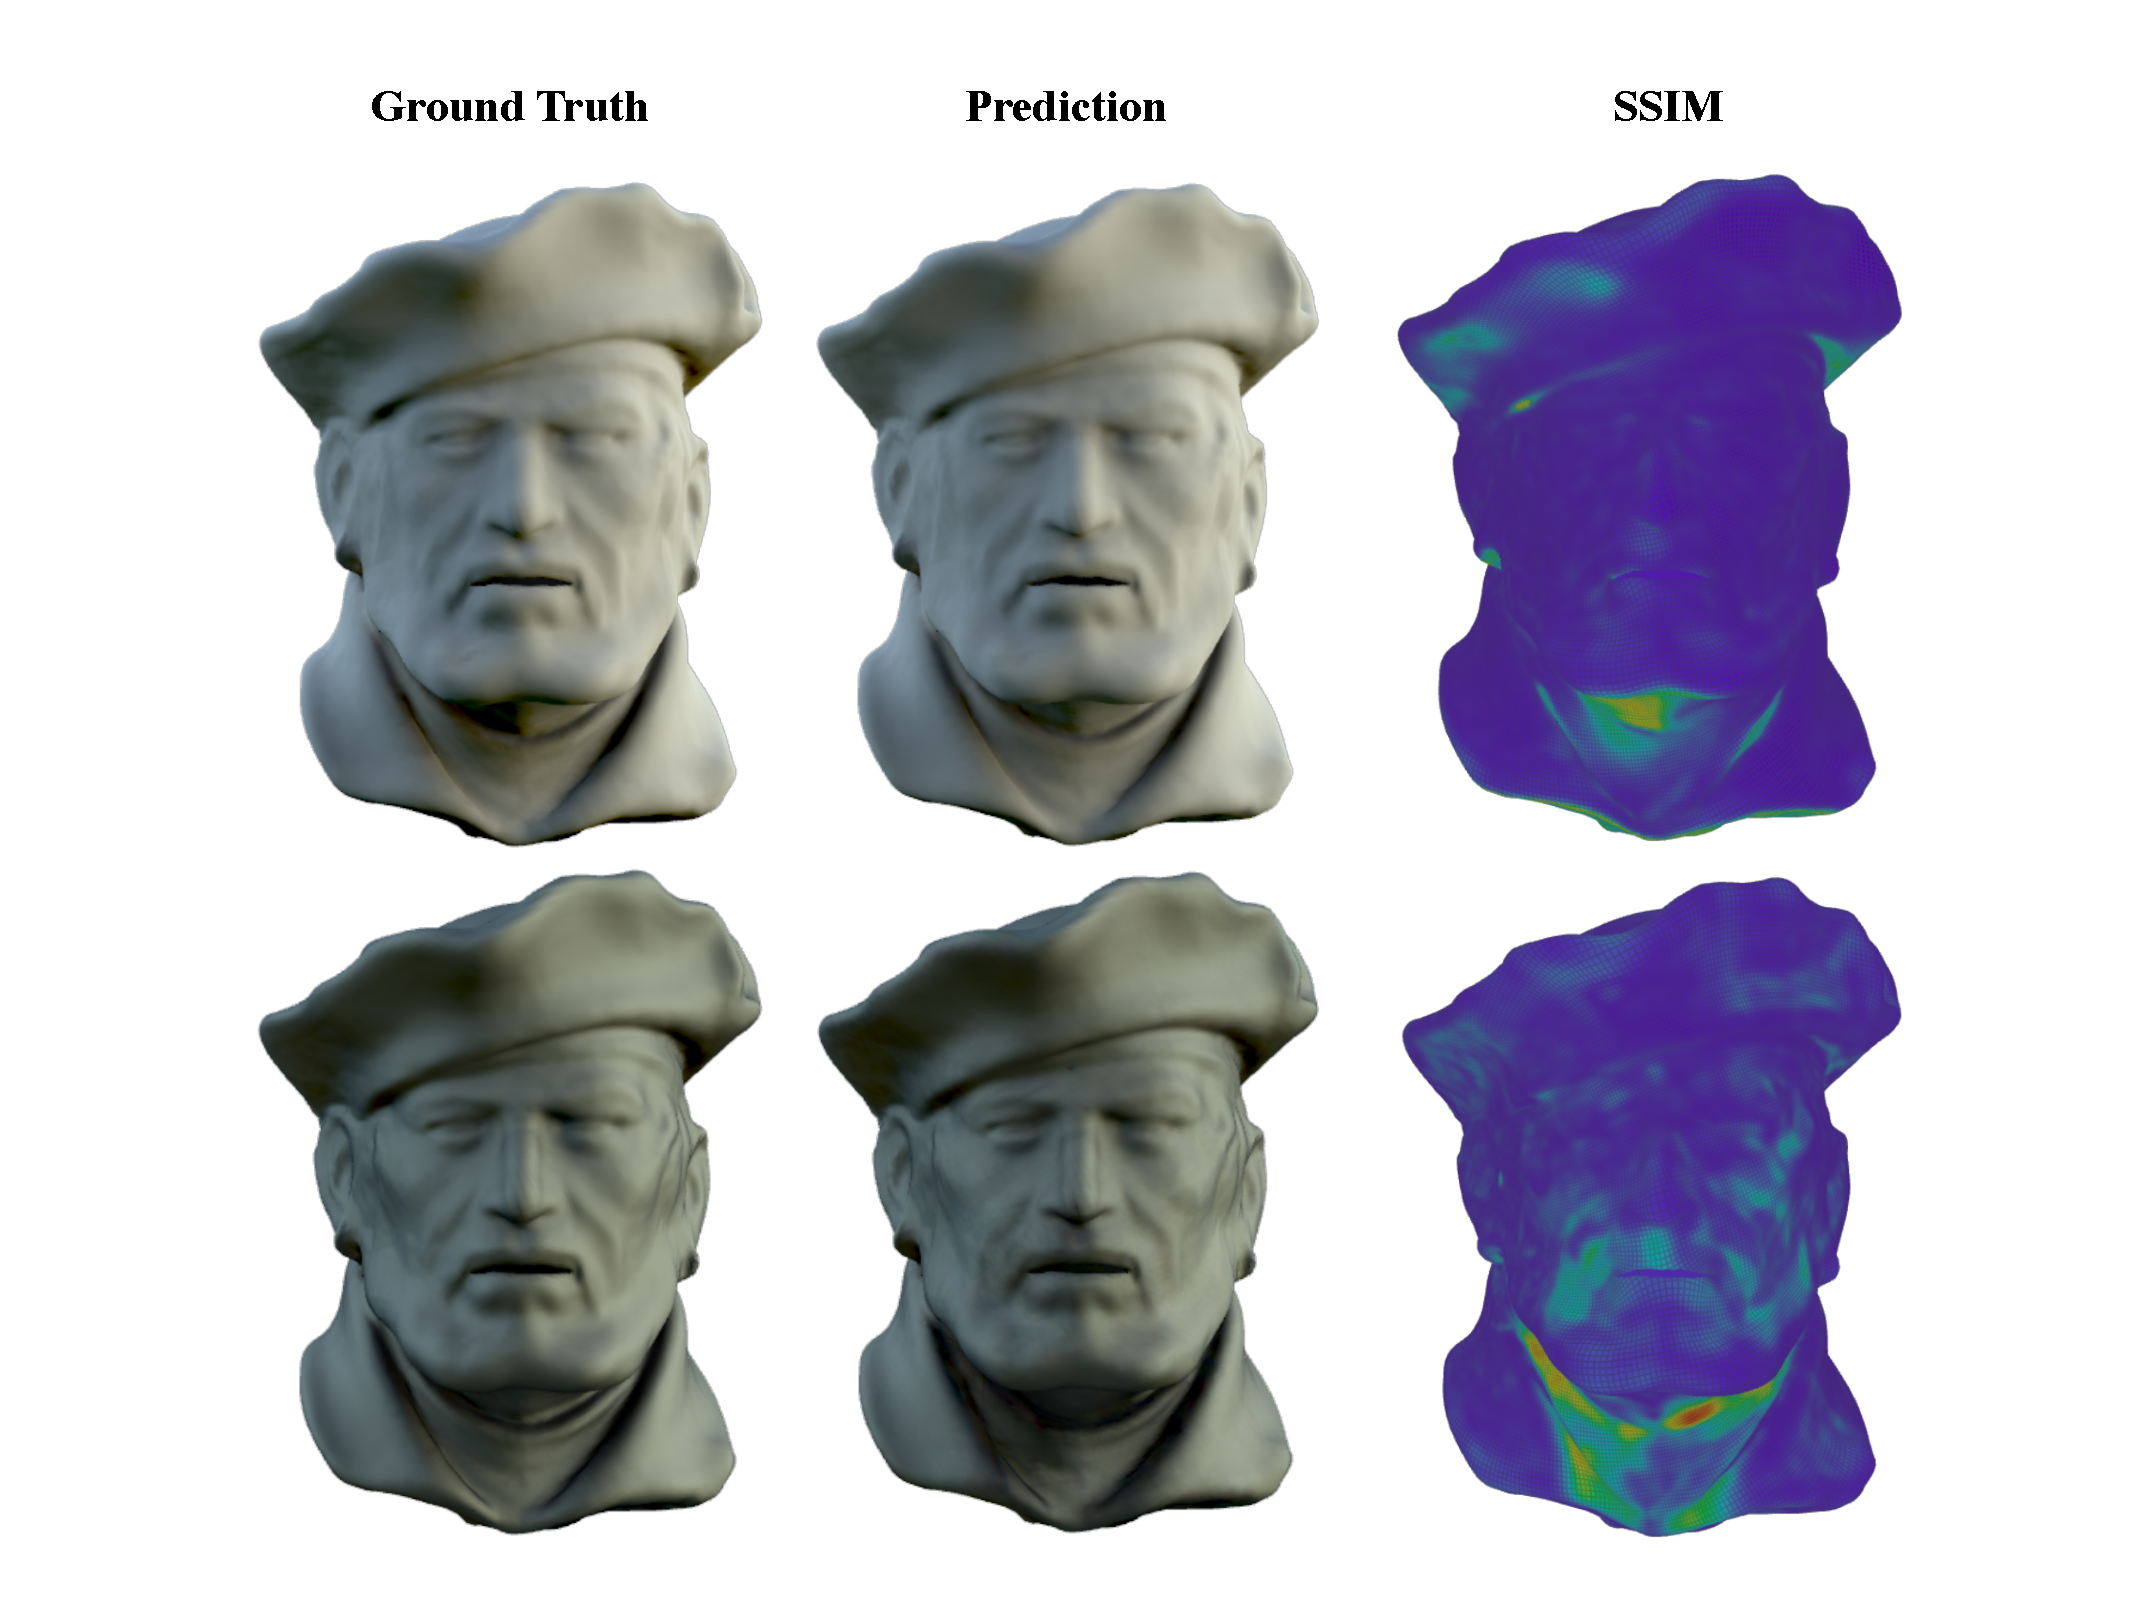
\includegraphics[width=0.35\textwidth]{Figures/glossy_pirate.pdf}
     \caption{Prediction of a test sample (unseen while training) for a diffuse (top) and glossy (bottom) surface. }
     \label{Fig: glossy_pirate}
\end{figure}
\subsubsection*{\textbf{Comparison with MoMoPRT}~:}
Furthermore, we compare our method with \cite{MoMoPRT} (MoMoPRT) and show that DeepPRT it is more accurate and can handle more general deformations. \\
The authors of \cite{MoMoPRT} proposed a linear model $f_{lin}$ to predict transfer coefficients from shape parameters of a \textit{morphable model}.
\\
Clearly, MoMoPRT is limited to shape deformations that are contained within the space described by a linear-shape-model $S_{lin}$. Moreover, although a linear model may be enough to approximate self-shadowing effects of shapes that are close to the mean shape of the data distribution of the training set, the model lacks complexity to accurately approximate data samples existing farther away from the mean shape (under-fitting).  
\\
On the other hand, our more complex non-linear model ($f_{CNN}$) is able to capture the relationships between the dataset's features (shape) and the target variable (transfer coefficients), enabling accurate approximations for a much larger deformation domain.\\
\\
For demonstration purposes, we generate a new training set consisting of $500$ shapes resulting from linear combinations between visually more dissimilar basis shapes\footnote{More distinguishable between each other, than between each face expressions used in \cite{MoMo}.}: 1) the \textit{Pirate Head } on one side, and 2)  a simple \textit{Plane} on the other. 
\begin{align*}
S_{lin} = \alpha ~ S_{pirate} + (1 - \alpha)~S_{plane}
\end{align*}
We train both models, $f_{CNN}$ and $f_{lin}$, and compute their predictions for a series of test-shapes that are evenly distributed. Figure (\ref{Fig:DPRT vs MoMoPRT A}) shows that the prediction accuracy of our $f_{CNN}$ model is higher and remains almost constant over the entire domain; on the contrary, the prediction accuracy of the linear model $f_{lin}$ drops significantly moving away from the mean shape (the \textit{Pirate/Plane} hybrid), as expected. 
\begin{figure}[h]
  \centering
    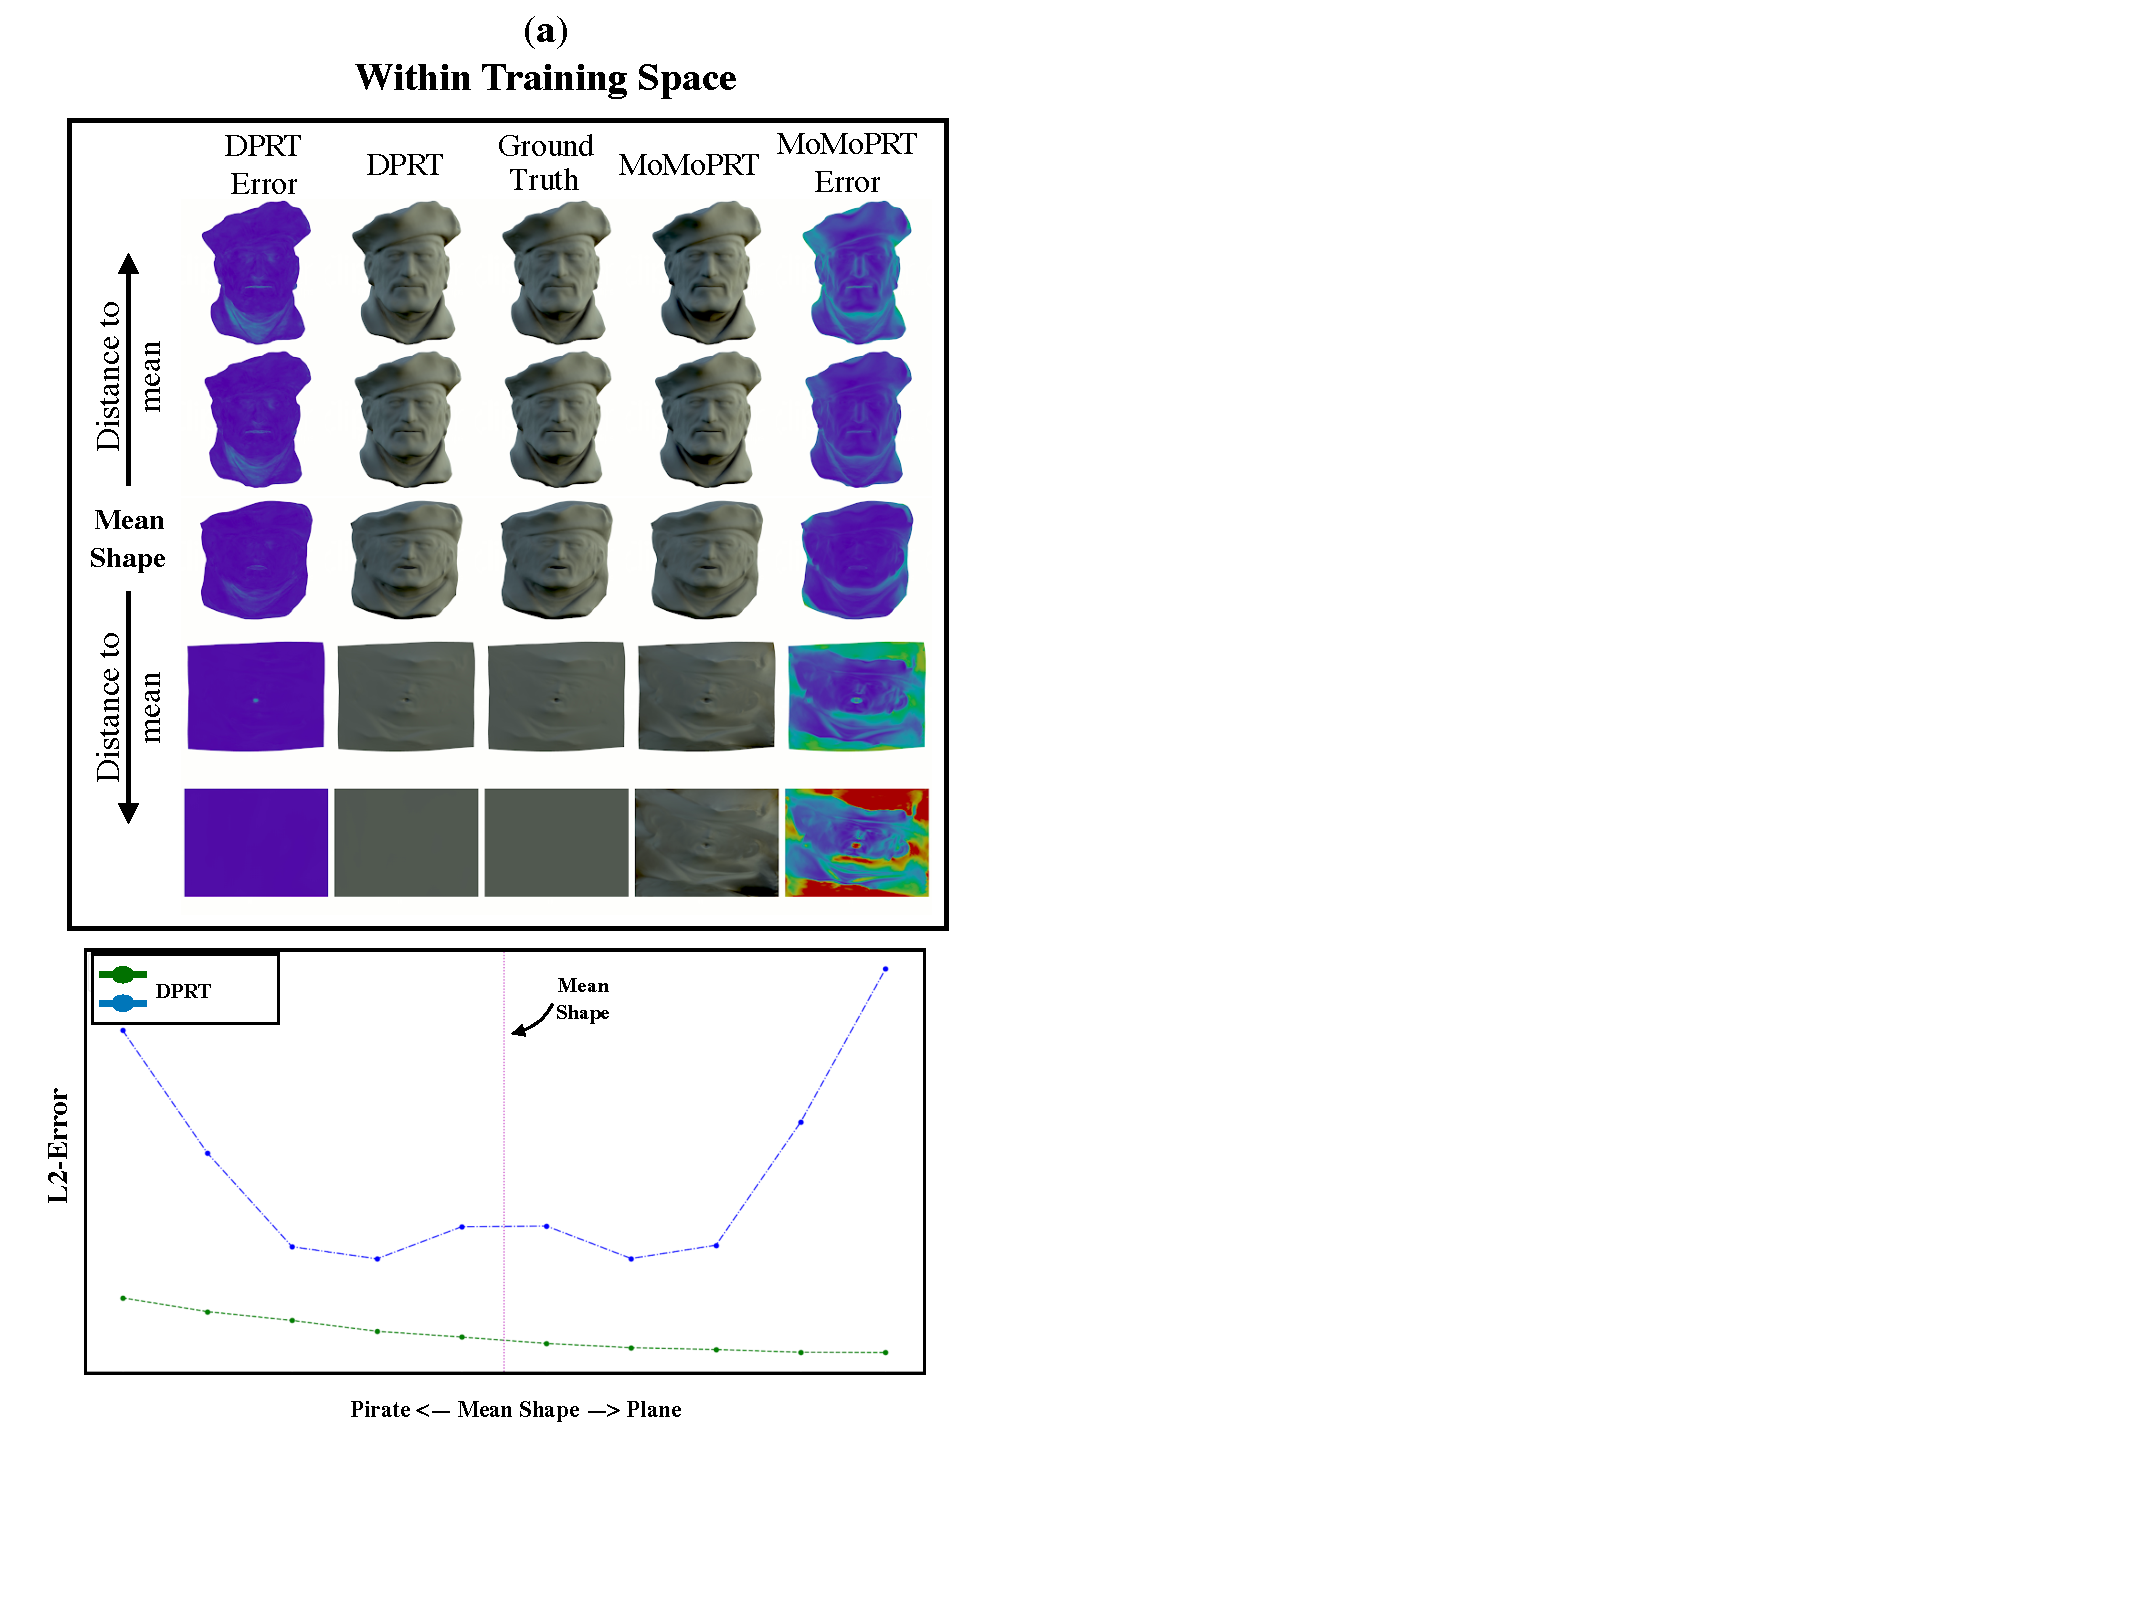
\includegraphics[width=0.4\textwidth]{Figures/DPRT_vs_MoMoPRT_a.pdf}
     \caption{DeepPRT (ours) vs. MoMoPRT, within training space.\textit{ Top:} Appearance and vertex-wise $L_2$-RGB distance between ground truth and predictions.\textit{ Bottom:} Plot of the mean $L_2$-RGB distance for each predicted shape. DeepPRT error is lower overall and close to constant, while MoMoPRT gets worse with increasing distance to mean shape.}
     \label{Fig:DPRT vs MoMoPRT A}
\end{figure}
Last but not least, we demonstrate that our model approximates data that is contained in a much larger domain than the one spanned by a linear-shape-model $S_{lin}$. The models, $f_{CNN}$ and $f_{lin}$, are fed with a series of sample shapes, starting from the mean shape and increasingly deforming towards a pirate face expression that was excluded from the training set. \\
As can be seen in Figure (\ref{Fig:DPRT vs MoMoPRT B}), the linear model performs poorly away from $S_{lin}$, while our network's accuracy remains constant.
\begin{figure}[h]
  \centering
    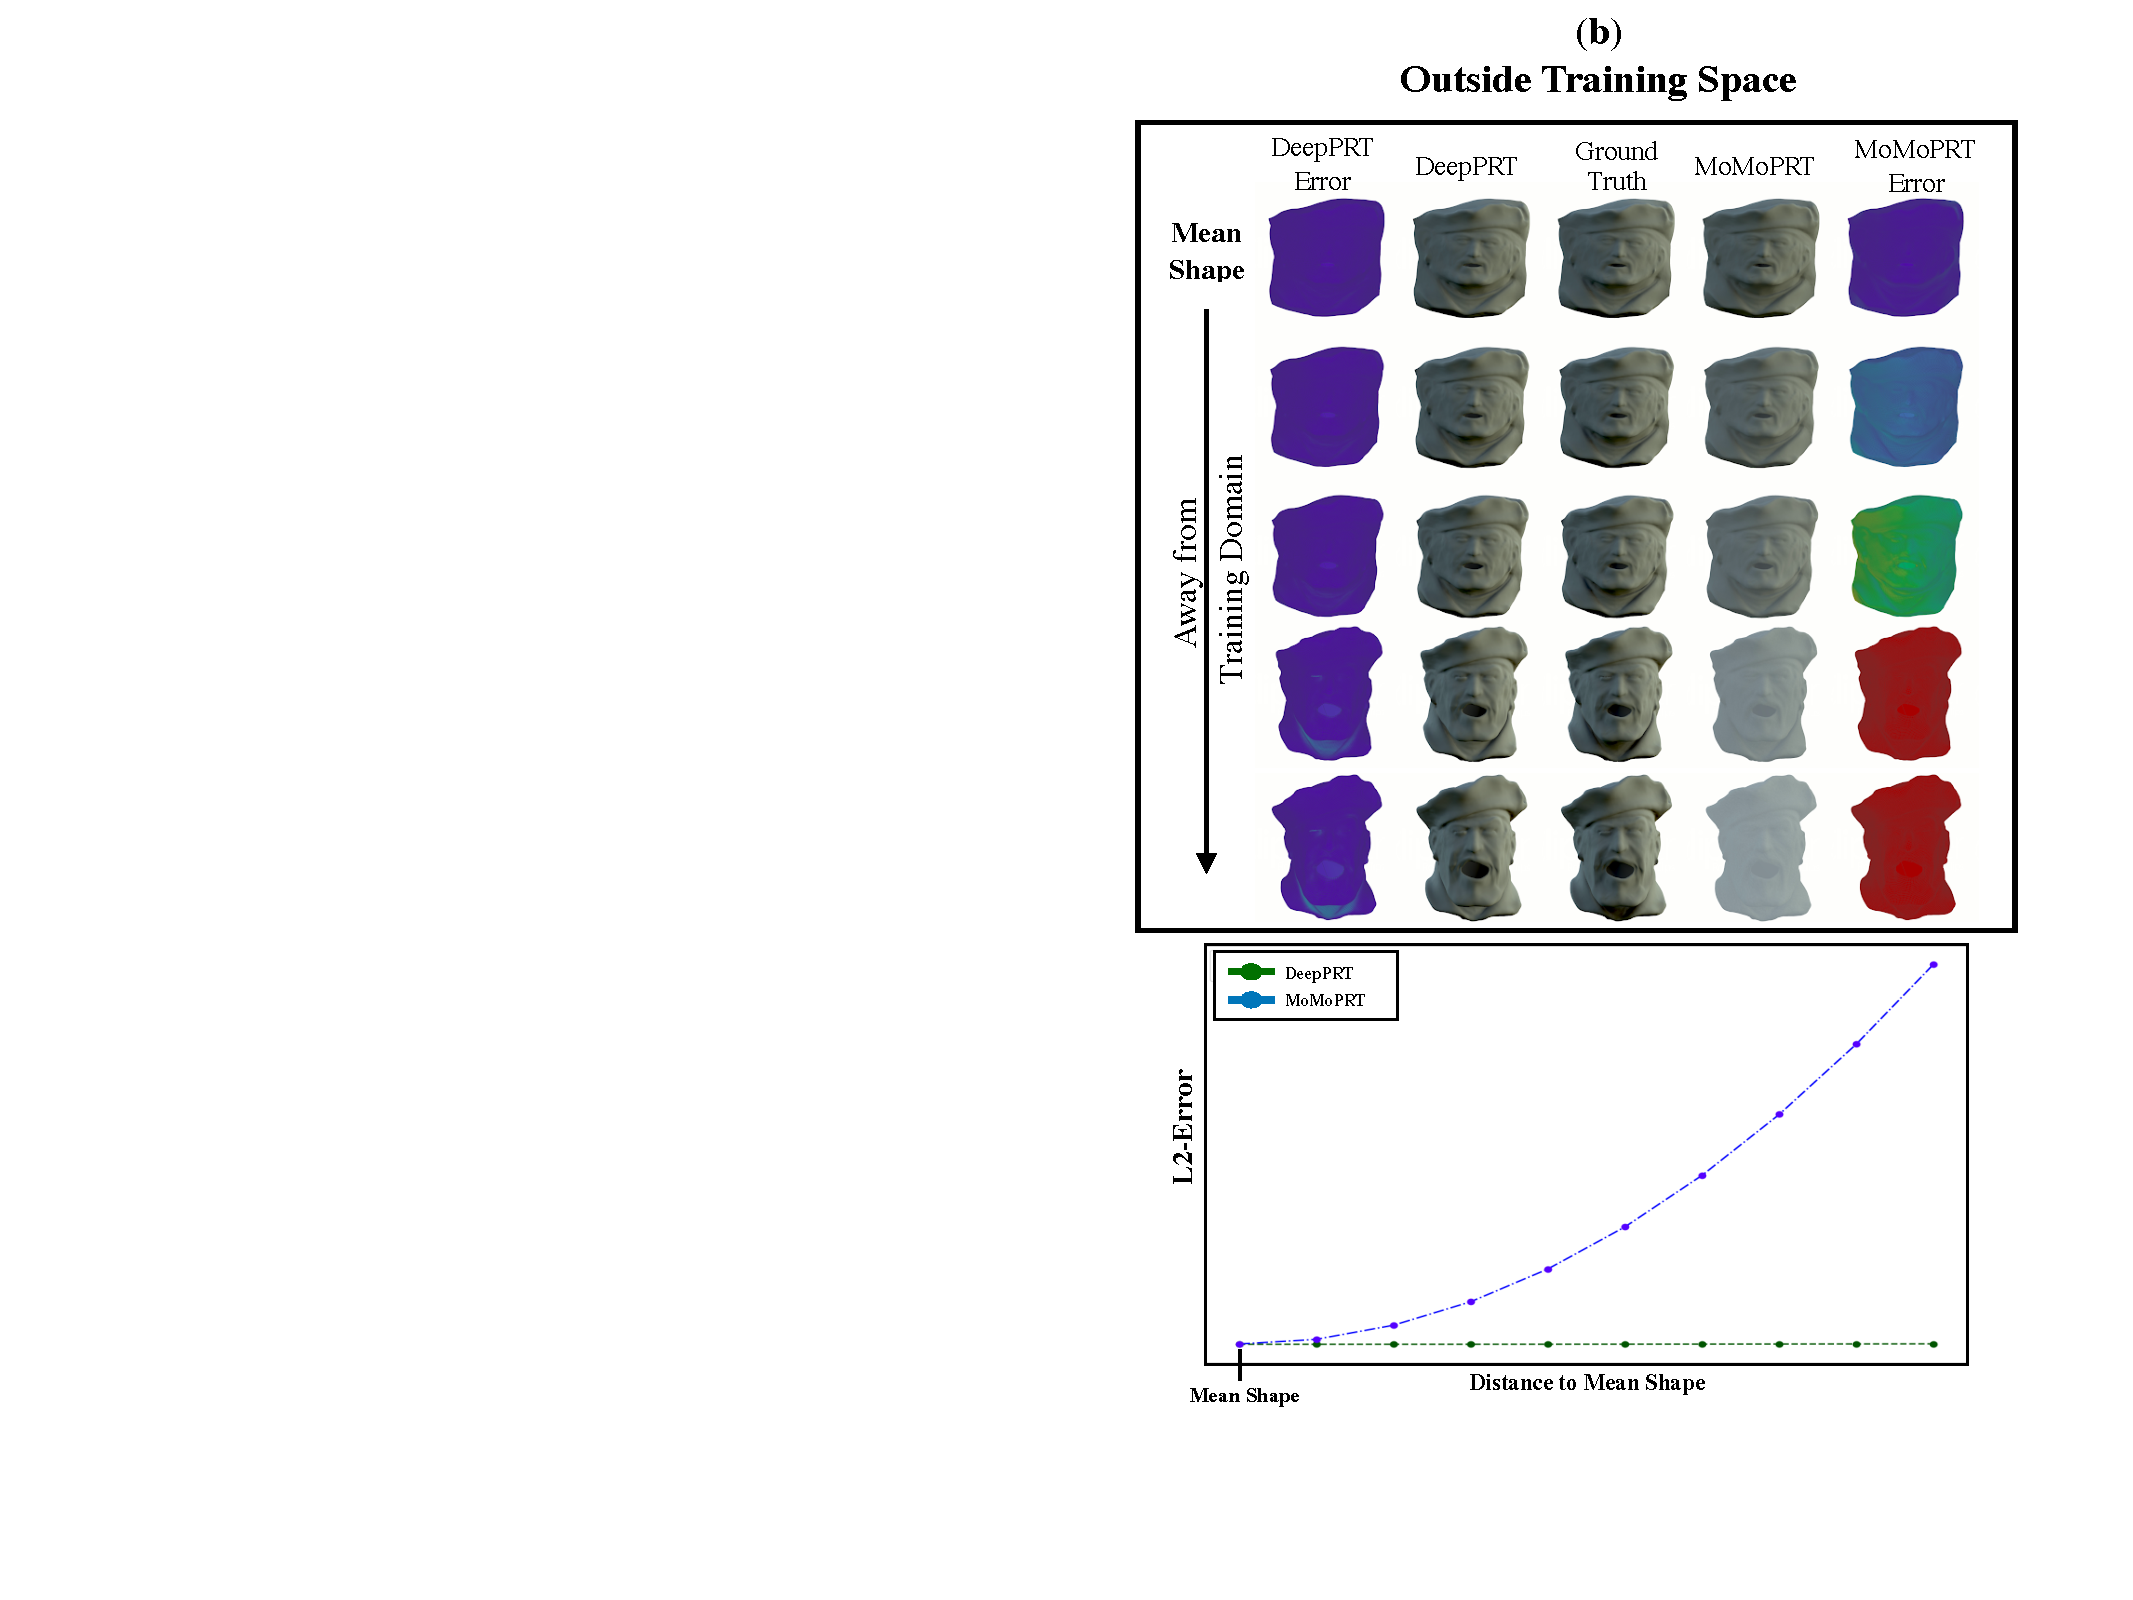
\includegraphics[width=0.4\textwidth]{Figures/DPRT_vs_MoMoPRT_b.pdf}
     \caption{DeepPRT (ours) vs. MoMoPRT, moving away from the training space. \textit{Top:} Appearance and vertex-wise $L_2$-RGB distance between ground truth and predictions.\textit{ Bottom:} Plot of the mean $L_2$-RGB distance for each predicted shape.}
     \label{Fig:DPRT vs MoMoPRT B}
\end{figure}

